\section{Fertige Landingpage}
Die Landingpage (siehe Abbildung \ref{fig:impl:finishedLandingpage}) repräsentiert das Projekt, denn es ist das erste, was ein neuer Benutzer*in von der Webanwendung zu sehen bekommt. Es war wichtig, ein modernes Design dafür zu entwickeln.

Wichtige Punkte, die bei der Landingpage beachtet wurden, waren die Hierarchie der Elemente. Zuerst gab es eine Einleitung, um das Projekt zu erklären, danach kam ein großer Knopf, der dazu einlädt, das Produkt zu verwenden. Er verlinkt zu der Anmeldung. Danach kam eine Selektion aus den neuesten erstellten Ausstellungen, damit kann sich der User gleich ein Bild vom Projekt machen.

\begin{figure}
    \centering
    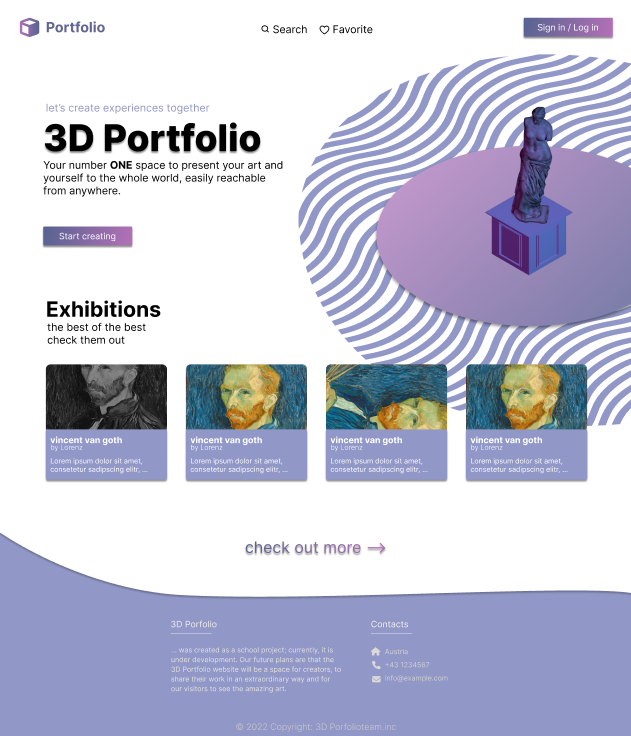
\includegraphics[scale=.5]{pics/startingpage.png}
    \caption{Landing Page}
    \label{fig:impl:finishedLandingpage}
\end{figure}

